\authoredSection{michael}{Aufgabenstellung und Vision}
	Die unser Gruppe übertragene Aufgabe bestand darin, eine iOS-App zu entwickeln, die die Bindung zwischen einer fiktiven Filialbank und ihren Kunden erhöht. In den ersten Ü\-ber\-le\-gung\-en wurde schnell deutlich, dass nahezu jede Dienstleistung einer Filiale auf die ein oder andere Weise von Direktbanken abgebildet werden kann. Das Alleinstellungsmerkmal besteht im direkten menschlichen Kontakt vor Ort und in der persönliche Bindung zu einem möglicherweise vertrauten Berater. 
    
    \begin{figure}
	\centering
	\begin{tabular}{@{}c@{\hspace{.5cm}}c@{}}
		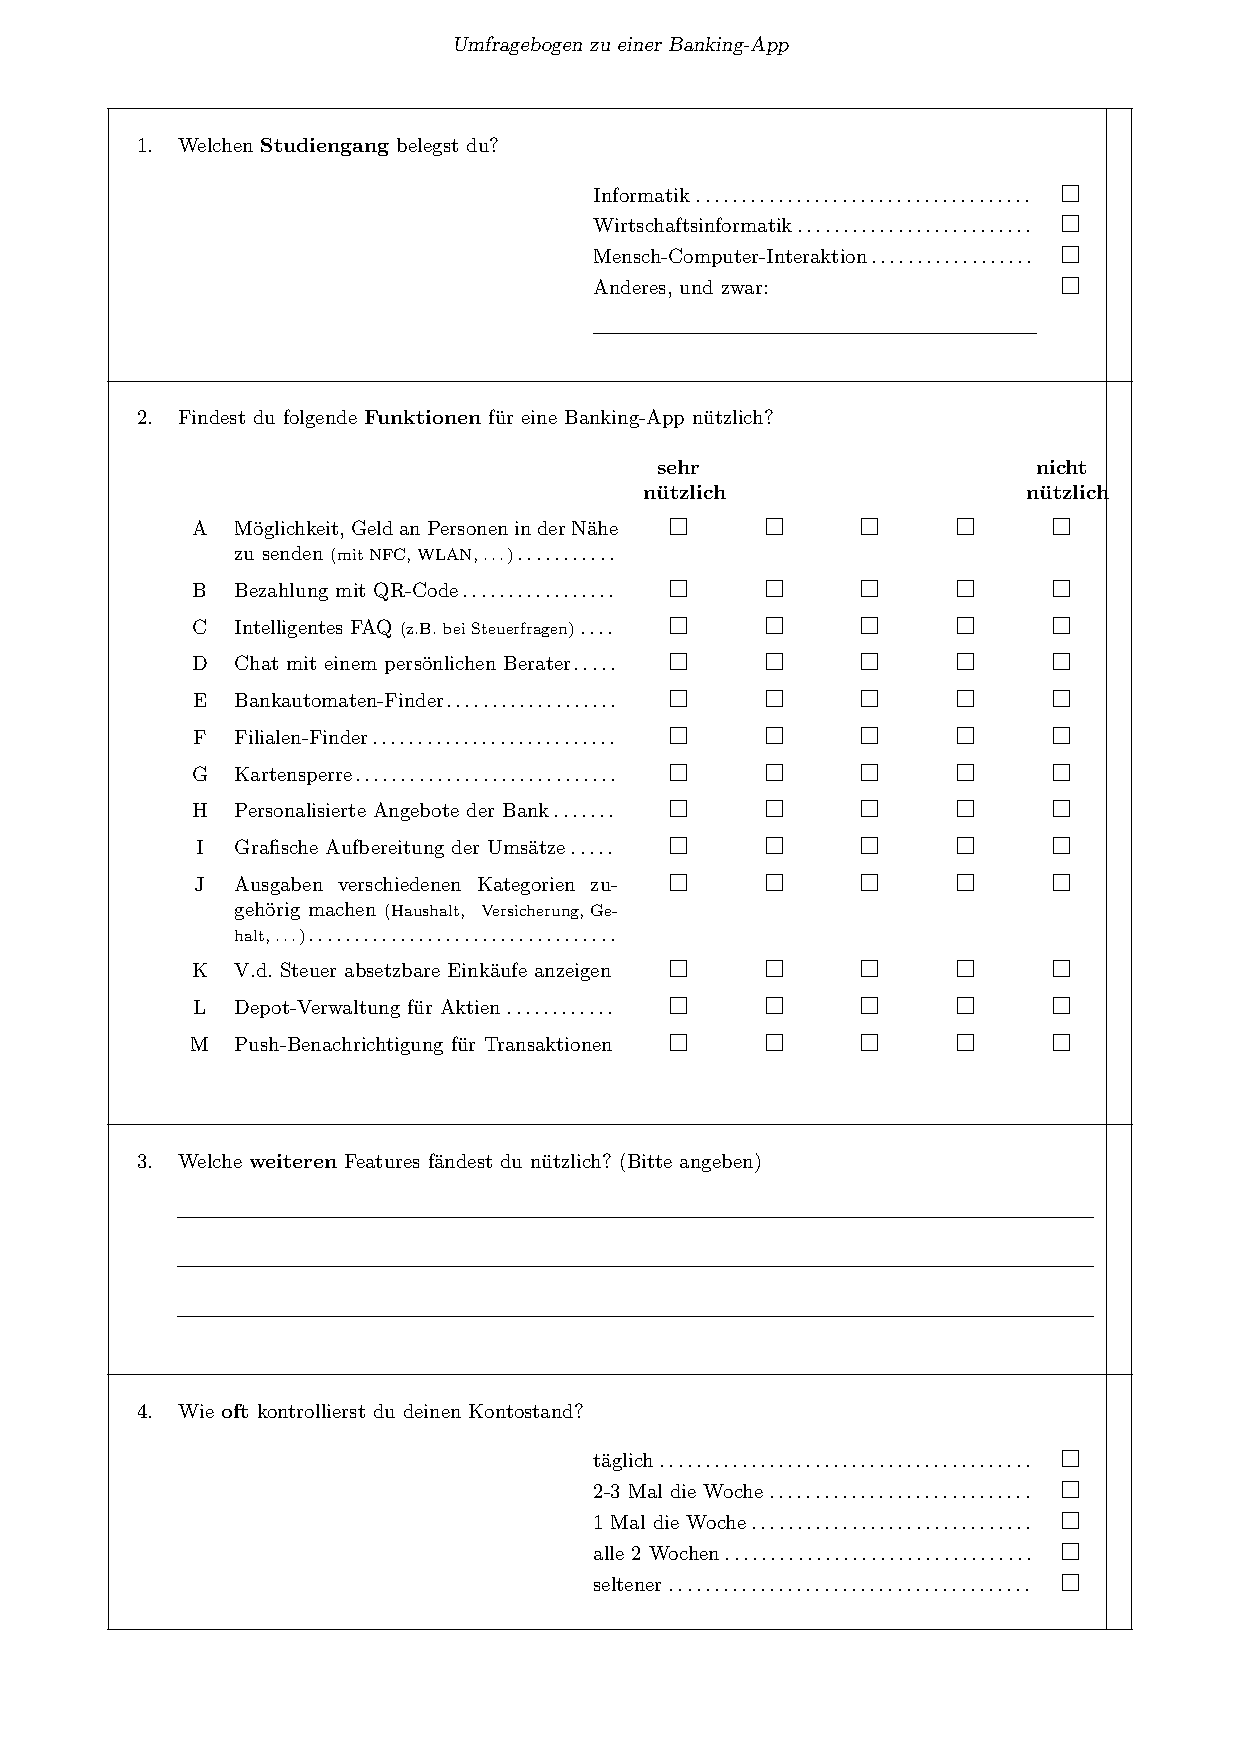
\includegraphics[page=1, height=110mm]{Pictures/Questionnaire} &
		\includegraphics[page=2, height=110mm]{Pictures/Questionnaire}
	\end{tabular}
	\label{fig:Questionnaire}
	\caption{Umfragebogen für erste Ist-Analyse}
\end{figure}


Insofern haben wir uns nach einem Prozess von abwechselnden Gruppendiskussion und externen Feedback dazu entschlossen, diejenigen Features zu betonen, die Berater und Kunden möglichst in der Filiale zusammenbringen, aber auch unabhängig davon genutzt werden können. Auch Direktbanken versuchen inzwischen, anonyme Hotlines zu vermeiden und Kunden einzelnen Beratern zuzuordnen. In Kombination mit niedrigeren Gebühren, kostenlosen Kreditkarten und einfacher Kontoführung ist dies ein schwer zu schlagendes Angebot. Eine App, die Neukunden für eine Filalbank gewinnen soll, muss also einerseits eine ähnlich einfache Kontoverwaltung bieten, außerdem aber noch einen Mehrwert schaffen, der die höheren Gebühren einer Filialbank rechtfertigt.

Ein weiterer, für die Akzeptanz einer App wichtiger Aspekt ist die (vielleicht auch nur vom Kunden gefühlte) Sicherheit. Eine von uns durchgeführte Umfrage unter Studenten technischer Fächer, primär Informatik, ergab, dass die meisten Teilnehmer unabhängig von der Funktionalität schon aus Sicherheitsgründen keine Bankgeschäfte mit einer App erledigen wollten. Die besondere Sensibilität der genannten Zielgruppe für Sicherheitsaspekte darf nicht außer Acht gelassen werden; dennoch ergab sich für uns die Frage, ob hier durch Interaktion in der Filiale nicht zugleich Kundenbindung und Vertrauen in die Sicherheit der Anwendung erhöht werden könnten. 

Insgesamt entstand also die Vorstellung einer Anwendung, die klassische Bankgeschäfte wie Überweisungen beherrscht, gleichzeitig aber versucht, Lokalität und Interaktion mit dem eigenen Berater herzustellen. 